\section{Исследовательская часть}

В текущем разделе будет поставлена цель эксперимента, проведён сам
эксперимент и сделаны соответствующие выводы.

\subsection{Технические характеристики}

Технические характеристики устройства, на котором выполнялось тестирование, представлены далее:

\begin{itemize}[leftmargin=1.6\parindent]
	\item[---] операционная система ~--- Windows 10 \cite{windows};
	\item[---] память ~--- 8 ГБ;
	\item[---] процессор ~--- 8 x AMD Ryzen 5 3500U \cite{amd}.
\end{itemize}

При тестировании ноутбук был включен в сеть электропитания. Во время тестирования ноутбук был нагружен только встроенными приложениями окружения, а также системой тестирования.

\subsection{Постановка эксперимента}

\subsubsection{Цель эксперимента}

Цель эксперимента -- выявить зависимость времени работы алгоритмов обработки изображений от разрешения изображений.

Время обработки изображения напрямую зависит от его разрешения, так как чем больше разрешение, тем больше будет матрица пикселей этого изображения.

\subsubsection{Проведение эксперимента}

Для проведения эксперимента были отобраны три изображения:

\begin{itemize}[leftmargin=1.6\parindent]
	\item[1)] изображение с низким разрешением (240х164);
	\item[2)] изображение со средним разрешением (512х640);
	\item[3)] изображение с высоким разрешением (1620х2160).
\end{itemize}

У всех трех изображений глубина цвета равняется 24 бит.

В таблице \ref{resTime} представлены результаты замеров времени (в мс) работы алгоритмов обработки изображений для трех типов, представленных выше.

\begin{table}[hbtp]
	\centering
	\begin{tabular}{|l||l|l|l|}
		\hline
		 & 240х164 & 512х640 & 1620х2160 \\
		\hline\hline 
		Негатив & 0.4879 & 4.569 & 43.3642 \\ \hline
		Оттенки	 серого & 0.4591 & 4.5026 & 47.0616 \\ \hline
		Размытие & 57.0516 & 510.937 & 5350.58 \\ \hline
		Снижение шума & 133.406 & 1125.05 & 11741.2 \\ \hline
		Яркость & 0.5155 & 4.4389 & 46.4873 \\ \hline
		Контрастность & 1.312 & 11.13 & 124.974 \\ \hline
	\end{tabular}
	\caption{\label{resTime} Результаты замеров времени}
\end{table}

Также, на рисунке \ref{img:graph1} и \ref{img:graph2} приведены графические результаты замеров работы алгоритмов в зависимости от разрешения исходного изображения.

\begin{figure}[hbtp]
	\centering
	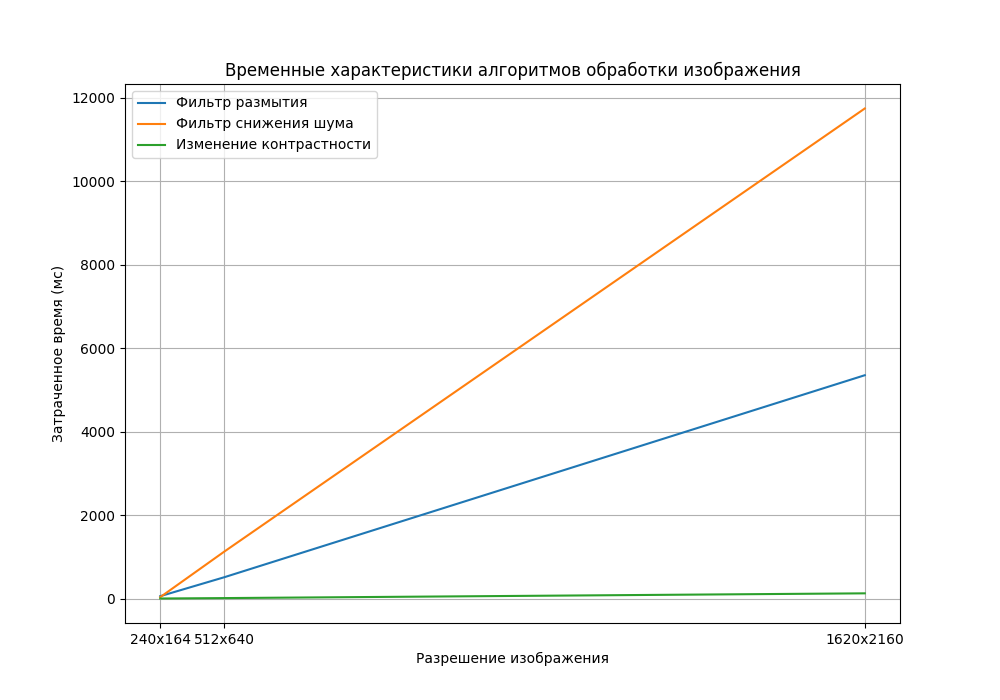
\includegraphics[width=0.9\textwidth]{img/graph1.png}
	\caption{\label{img:graph1} Замеры времени -- 1}
\end{figure}

\begin{figure}[hbtp]
	\centering
	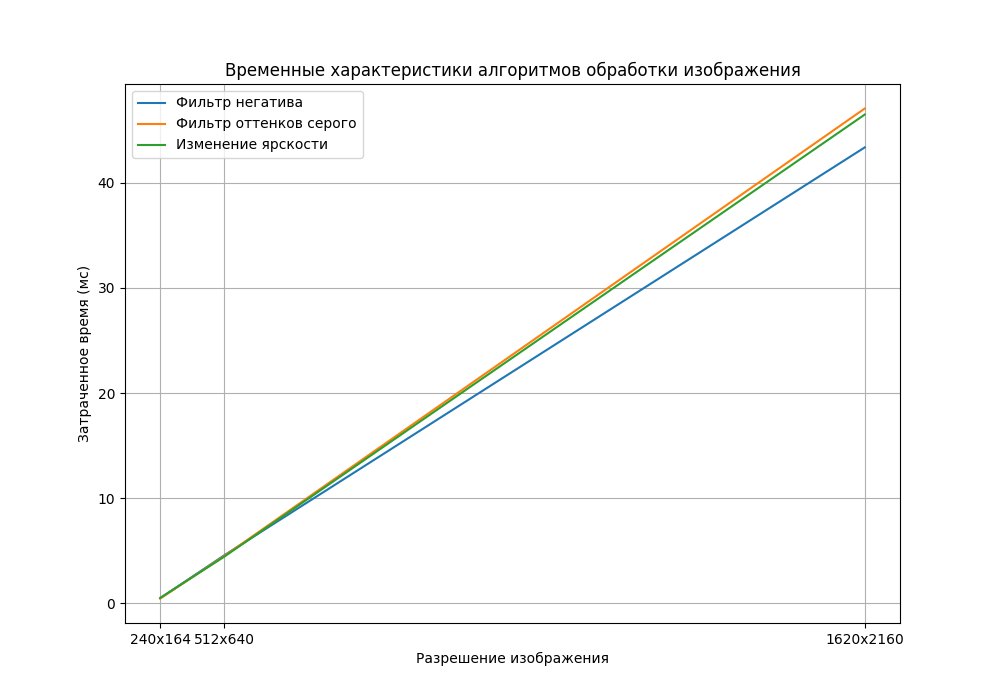
\includegraphics[width=0.9\textwidth]{img/graph2.png}
	\caption{\label{img:graph2} Замеры времени -- 2}
\end{figure}

\subsection*{Вывод}
Исходя из полученных результатов, можно сделать вывод, что время работы любого алгоритма обработки изображений (из представленных в данной работе) линейно зависит от разрешения этого изображения. При увеличении разрешения в 10 раз -- время работы алгоритмов также увеличивается в 10 раз.

Также, можно отметить, что алгоритмы, основанные на матрице свертки работаю дольше, чем точечные. Это обуславливается тем, что при применении точечного фильтра каждый пиксель обрабатывается ровно один раз, а при применении матрицы свертки -- 9 раз.

\pagebreak